\hfill \smallbreak
Kada želimo uspostaviti vlastiti besplatan VPN, jedna opcija je ugrađeni VPN koji Windows 10 ima. Slijede korak po korak upute kako izraditi i uspostaviti vlastiti VPN server. Napomena: VPN server se nalazi u mreži kojoj kasnije želimo pristupati koristeći udaljeno računalo klijent.  
\smallbreak
\subparagraph{1. Korak:  moramo računalu dodijeliti statičku lokalnu IP adresu}
\hfill \smallbreak
Otvorimo Postavke, Mreža i Internet, u izborniku s lijeve strane Ethernet i naposljetku opciju Promjena mogućnosti prilagodnika. Nakon toga dobili smo prozor poput onog na slici 1.
\begin{figure}[h!]
	\centering
     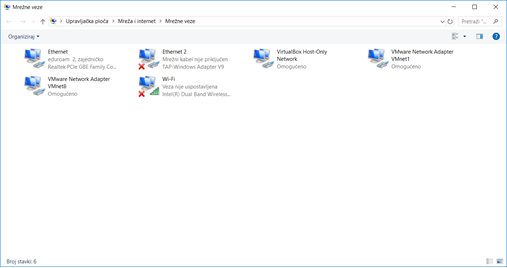
\includegraphics[width=0.8\textwidth]{Win10/Slika1}
     \caption{Prozor Promjena mogućnosti prilagodnika}
\end{figure}
\FloatBarrier
Ovdje nam je bitna samo ikona Ethernet, otvorit ćemo ju desnim klikom miša te odabrati Stanje, Detalji… i dobit ćemo prozor sa slike 2.
\begin{figure}[h!]
	\centering
     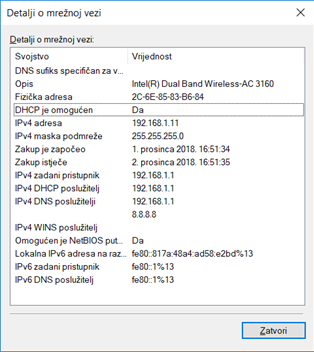
\includegraphics[width=0.5\textwidth]{Win10/Slika2}
     \caption{Prozor Detalji o mrežnoj dijagnostici}
\end{figure}
\FloatBarrier
Pogledamo podatke o IPv4 adresi, maski podmreže, zadanom pristupniku i DNS poslužitelju, zapamtimo te brojeve i moramo ih upisati kada zatvorimo trenutni prozor i u prošlom prozoru gdje smo otvorili detalje sada otvorimo Svojstva te odaberemo stavku Internet Protocol Version 4 (TCP/IPv4) te ponovno odaberemo Svojstva. U novom prozoru koji smo dobili ponovno nam trebaju oni brojevi koje smo zapamtili(IP adresa) i s njima popunimo podatke kao na slici 3.
\begin{figure}[h!]
	\centering
     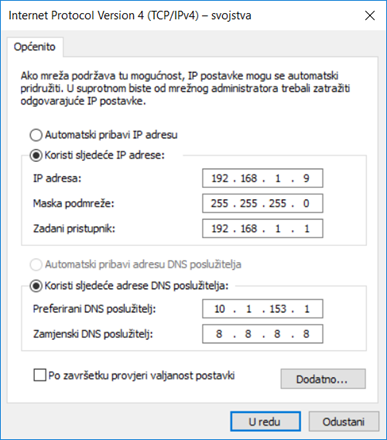
\includegraphics[width=0.5\textwidth]{Win10/Slika3}
     \caption{Svojstva (IPv4)}
\end{figure}
\FloatBarrier
Kliknemo U redu i gotovi smo s prvim korakom.
\FloatBarrier
\newpage
\subparagraph{2. Korak: Postaviti VPN server}
\hfill \smallbreak
Vratimo se u prozor Promjena mogućnosti prilagodnika sa Slike 1, tamo pritisnemo tipku Alt te u alatnoj traci koja se pojavila odaberemo karticu Datoteka, Nova dolazna veza.
U dobivenom prozoru odaberemo Dodaj osobu te popunimo prozor Novi korisnik po želji, ali pazeći pri tome da lozinka bude jaka (kombinacija brojeva, velikih i malih slova).
\FloatBarrier
\begin{figure}[h!]
	\centering
     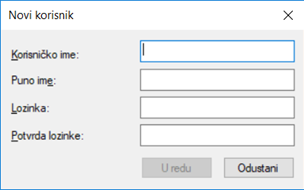
\includegraphics[width=0.4\textwidth]{Win10/Slika4}
     \caption{Prozor Novi korisnik}
\end{figure}
\FloatBarrier
Nakon toga označimo stvoreni profil i odaberemo Dalje, u novom prozoru označimo kvačicom opciju koju nam nudi te ponovno stisnemo Dalje. U sljedećem koraku kliknemo Dopusti pristup ako su polja označena kao na slici 5.
\FloatBarrier
\begin{figure}[h!]
	\centering
     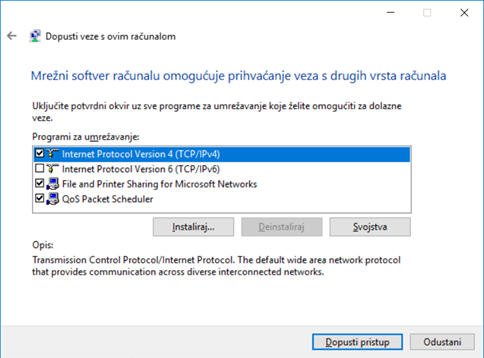
\includegraphics[width=0.8\textwidth]{Win10/Slika5}
     \caption{Dopusti veze s ovim računalom}
\end{figure}
\FloatBarrier
Dobili smo prozor koji prikazuje ime računala koje će nam trebati kasnije da se spojimo na naš VPN.
\FloatBarrier
\newpage
\subparagraph{3. Korak: Postaviti usmjeritelj da prosljeđuje priključak 1723}
\hfill \smallbreak
Pristupimo postavkama usmjeritelja i postavimo prosljeđivanje porta 1723 kao što je opisano u poglavlju 5, pri čemu upisujemo podatke kao sa slike 6. Ako ne znamo korisničko ime i lozinku, a nismo ih mijenjali možemo pronaći pretpostavljene za svaki usmjeritelj na stranici \url{https://portforward.com/router-password/}. 
\FloatBarrier
\begin{figure}[h!]
	\centering
     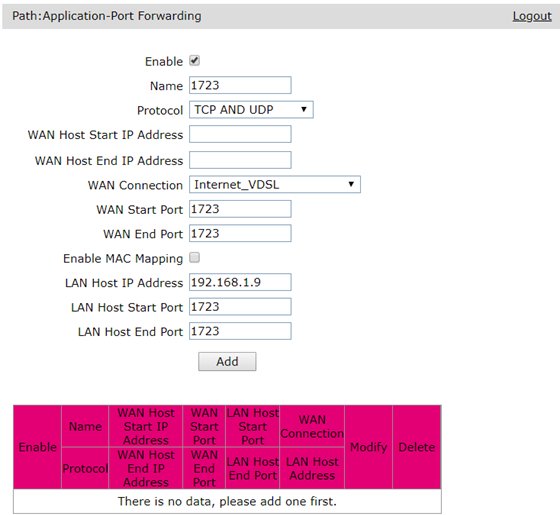
\includegraphics[width=0.8\textwidth]{Win10/Slika6}
     \caption{Postavke usmjeritelja za prosljeđivanje}
\end{figure}
\FloatBarrier
\subparagraph{4. Korak: Postavke Vatrozida za VPN promet}
\hfill \smallbreak
Na Upravljačkoj ploči odaberemo Vatrozid, Dodatne postavke, Inbound Rules, New Rule. U prozoru koji se otvori odaberemo Port i stisnemo Next. Na slikama 7., 8. i 9. vidimo kako trebaju izgledati sljedeći prozori. Kada ih popunimo tako kliknemo Next.
\FloatBarrier
\begin{figure}[h!]
	\centering
     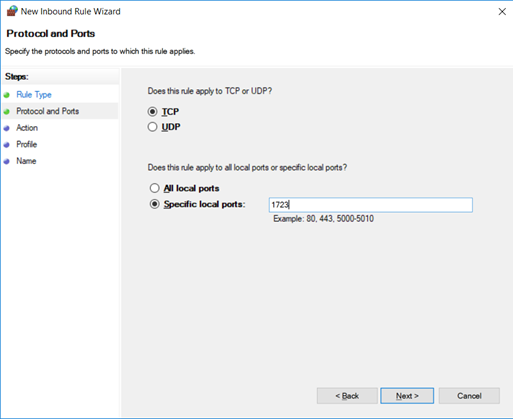
\includegraphics[width=0.8\textwidth]{Win10/Slika7}
     \caption{Dodavanje pravila za port 1723}
\end{figure}
\FloatBarrier
\FloatBarrier
\begin{figure}[h!]
	\centering
     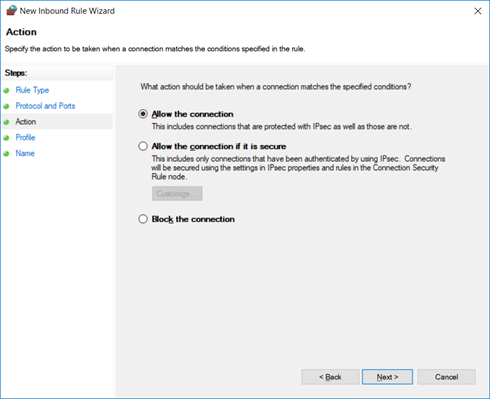
\includegraphics[width=0.8\textwidth]{Win10/Slika8}
     \caption{Dopuštanje veze}
\end{figure}
\FloatBarrier
\FloatBarrier
\begin{figure}[h!]
	\centering
     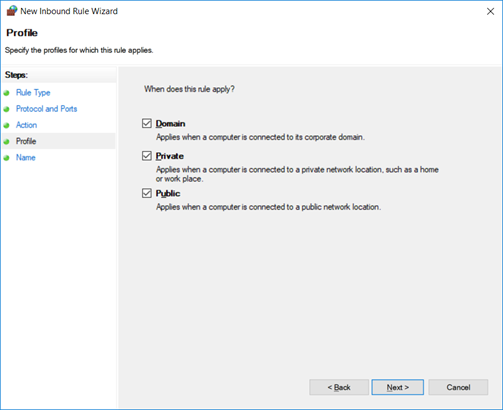
\includegraphics[width=0.8\textwidth]{Win10/Slika9}
     \caption{Odabir kada se pravilo primjenjuje}
\end{figure}
\FloatBarrier
U sljedećem prozoru za ime napišemo 1723, a polje za opis možemo i ostaviti prazno te odaberemo Finish. Sada ponovno odaberemo New Rule i sve ponovimo osim što u prozoru sa slike 7. odaberemo UTP te u zadnjem koraku odaberemo različito ime, npr. 1723udp. Sada na stranici \url{https://www.yougetsignal.com/tools/open-ports/} testiramo je li port 1723 zaista otvoren i ako dobijemo poruku da je sve u redu, gotovi smo s korakom 4.
\FloatBarrier
\subparagraph{5. Korak: Postavljanje domene}
\hfill \smallbreak
Na stranici \url{https://www.noip.com/} izradimo besplatan račun i odaberemo slobodnu domenu koju ćemo lako zapamtiti. Sada je naša javna IP-adresa povezana s imenom domene. Nakon aktivacije računa trebamo skinuti i instalirati Dynamic DNS Update Client ( \url{https://www.noip.com/download?page=win}) koji stalno provjerava promjene vezane za IP-adresu. U zadnjem koraku instalacije označimo obadvije kućice (Launch i Run DUC as System Service in the background). Nakon instalacije otvori se prostor za prijavu pa se prijavimo s podacima s kojima smo izradili račun. Označimo kućicu kraj imena stvorene domene i odaberemo Save te dobijemo prozor kao na slici 10. 
\FloatBarrier
\FloatBarrier
\begin{figure}[h!]
	\centering
     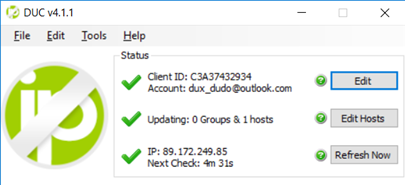
\includegraphics[width=0.6\textwidth]{Win10/Slika10}
     \caption{DUC}
\end{figure}
\FloatBarrier
\subparagraph{Povezivanje na VPN}
\hfill \smallbreak
Sada je sve spremno za povezivanje na naš VPN server. Na udaljenom računalu klijentu otvorimo Centar za mreže i zajedničko korištenje, Postavljanje nove veze ili mreže, Povezivanje s radnim mjestom, Koristi internetsku vezu (VPN). U prozoru na Slici 11 za polje Internetska adresa možemo upisati domenu ili javnu IP-adresu.
\FloatBarrier
\begin{figure}[h!]
	\centering
     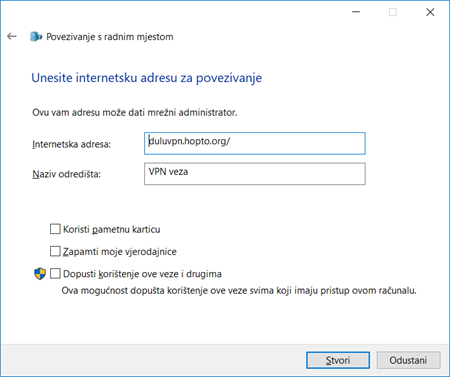
\includegraphics[width=0.8\textwidth]{Win10/Slika11}
     \caption{Adresa povezivanja}
\end{figure}
\FloatBarrier
I zadnja stvar koju treba napraviti je na klijentskom računalu u postavkama mreže i interneta odabrati VPN vezu te upisati korisničko ime i lozinku iz drugog koraka i nakon toga smo povezani na naš VPN server, što znači da računalo klijent ima IP-adresu kao da se nalazi u mreži u kojoj je računalo server.

\FloatBarrier